\clearpage
\section{Electrical Connections and Onboard I/O}
\label{sec:electrical-design}
\subsection{Shared Battery and Two Power Rails}
The recorded wiring uses one shared two-cell 18650 pack (2S, 7.4\,V nominal), with separate 5\,V logic and 6\,V motor buck converters. S1 enables the logic branch and feeds the downstream S2 motor switch. Opening S2 removes motor power while leaving computing and sensing powered. Desktop and ASUS use their own external supplies.

\begin{figure}[H]
\centering
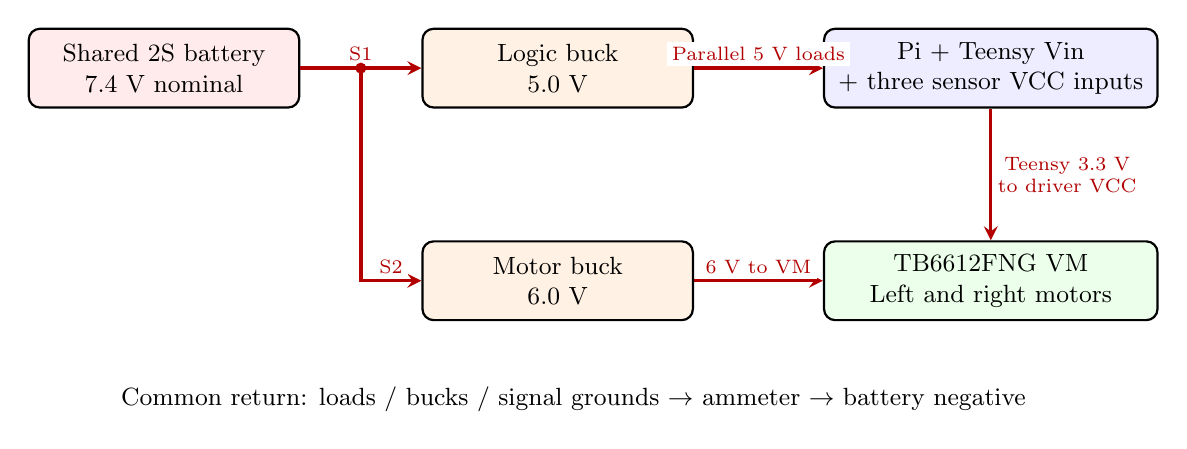
\begin{tikzpicture}[font=\small,>=stealth,
 block/.style={draw,thick,rounded corners,align=center,text width=3.2cm,minimum height=1cm},
 rail/.style={->,very thick,red!70!black},
 note/.style={font=\scriptsize,fill=white,align=center,inner sep=2pt}]
\node[block,fill=red!8] (pack) at (0,4) {Shared 2S battery\\7.4 V nominal};
\node[block,fill=orange!10] (logic) at (5,4) {Logic buck\\5.0 V};
\node[block,fill=orange!10] (motor) at (5,1.3) {Motor buck\\6.0 V};
\node[block,fill=blue!7,text width=4cm] (loads) at (10.5,4) {Pi + Teensy Vin\\+ three sensor VCC inputs};
\node[block,fill=green!8,text width=4cm] (driver) at (10.5,1.3) {TB6612FNG VM\\Left and right motors};
\draw[rail] (pack) -- node[note,above] {S1} (logic);
\draw[rail] (2.5,4) -- (2.5,1.3) -- node[note,above] {S2} (motor);
\fill[red!70!black] (2.5,4) circle (2pt);
\draw[rail] (logic) -- node[note,above] {Parallel 5 V loads} (loads);
\draw[rail] (motor) -- node[note,above] {6 V to VM} (driver);
\draw[rail] (loads) -- node[note,right] {Teensy 3.3 V\\to driver VCC} (driver);
\node[align=center,font=\small] at (5.2,-.2) {Common return: loads / bucks / signal grounds $\to$ ammeter $\to$ battery negative};
\end{tikzpicture}

\caption{Current power topology. One battery feeds two converters; this replaces the earlier independent-power-bank concept. Grounds join on the load side of the return ammeter. Pi--Teensy control data uses 3.3\,V UART, not USB CDC.}
\label{fig:power_topology}
\end{figure}

The 5\,V output feeds Pi, Teensy Vin and all three sensor VCC inputs in parallel. Teensy's USB power bridge is cut to isolate VUSB from Vin. Teensy 3.3\,V feeds TB6612FNG VCC; the 6\,V buck feeds VM. Motor leads connect across each bridge's two outputs, not to ground. Converter capacity, motor stall current and pack discharge performance remain uncharacterized in this record.

All signal grounds share a reference. Route motor current back to the motor buck rather than through Teensy or sensor ground leads. The detailed diagram omits charging/protection and bypass components. Retain the documented local bypassing and motor suppression; the earlier recommendation was a 470--1000\,$\mu$F motor-rail bulk capacitor and 0.1\,$\mu$F across each motor, not a measured inventory of fitted parts.

\clearpage
\subsection{Pi, Teensy and Motor-Driver Wiring}
\begin{figure}[H]
\centering
\resizebox{.86\linewidth}{!}{% Editable electrical connection diagram; coordinates in cm.
\begin{circuitikz}[american,font=\small,
  logic/.style={draw=blue!65!black,fill=blue!5,thick},
  powerwire/.style={draw=red!75!black,very thick,>=stealth},
  motorwire/.style={draw=magenta,very thick},
  signalwire/.style={draw=blue!65!black,thick},
  pintext/.style={font=\scriptsize},
  smallnote/.style={font=\scriptsize,align=center}]
\ctikzset{diodes/scale=0.55,resistors/scale=0.55}
% Stacked cells: series link on the right, pack leads on the left.
\draw[thick,fill=red!6] (2.1,13.5) rectangle (3.9,14.3);
\draw[thick,fill=red!6] (2.1,12.5) rectangle (3.9,13.3);
\node[smallnote] at (3,13.9) {Cell 1\\3.7 V};
\node[smallnote] at (3,12.9) {Cell 2\\3.7 V};
\node[pintext] at (2.3,13.9) {$-$}; \node[pintext] at (3.7,13.9) {$+$};
\node[pintext] at (2.3,12.9) {$+$}; \node[pintext] at (3.7,12.9) {$-$};
\draw[powerwire,->] (3.9,13.9) -- (4.3,13.9) -- (4.3,12.9) -- (3.9,12.9);
% Horizontal cylindrical connector to the left of the cells.
\draw[thick,fill=gray!10] (1,13.71) -- (0.2,13.71)
  arc[start angle=90,end angle=270,x radius=0.12,y radius=0.36]
  -- (1,12.99) -- cycle;
\draw[thick,fill=gray!20] (1,13.35) ellipse[x radius=0.12,y radius=0.36];
\node[pintext] at (0.6,13.55) {$-$};
\node[pintext] at (0.6,13.15) {$+$};
\node[pintext] at (0.6,14.0) {Plug};
\draw[thick] (2.1,13.9) -- (1.5,13.9) -- (1.5,13.55) -- (1,13.55);
\draw[powerwire,->] (2.1,12.9) -- (1.7,12.9) -- (1.7,13.15) -- (1,13.15);
\draw[powerwire] (0.2,13.15) -- (0,13.15) -- (0,12.3) -- (4.5,12.3);
\node[circle,draw,thick,minimum size=0.7cm,inner sep=0pt] (batteryammeter) at (-0.4,11.1) {A};
\draw[thick] (0.2,13.55) -- (-0.4,13.55) -- (batteryammeter.north);
\draw[thick] (batteryammeter.south) -- (-0.4,9.9) node[ground] {};
\node[smallnote,anchor=west] at (0.15,11.1) {Battery return\\ammeter};
\node[smallnote] at (2.4,14.8) {Shared Li-ion battery: two cells in series\\7.4 V nominal (2S)};
% S1 enables the logic branch; S2 additionally enables the motor branch.
\draw[logic,fill=orange!8] (4.25,9.6) rectangle (6.85,10.8);
\node[smallnote] at (5.55,10.2) {Logic buck\\OUT: 5.0 V};
\draw[logic,fill=orange!8] (10.2,9.6) rectangle (12.8,10.8);
\node[smallnote] at (11.5,10.2) {Motor buck\\OUT: 6.0 V};
\draw[powerwire] (4.5,12.3) to[nos] (7,12.3);
\node[smallnote] at (5.75,13.05) {S1: main / logic\\toggle switch};
\draw[powerwire,->] (7,12.3) to[nos] (10.2,12.3) -- (11.5,12.3) -- (11.5,10.8);
\node[smallnote] at (8.6,13.05) {S2: motors\\toggle switch};
\draw[powerwire,->] (7,12.3) node[circ] {} -- (7,11.5) -- (5.55,11.5) -- (5.55,10.8);
\node[pintext,anchor=west] at (5.7,11.1) {IN+};
\node[pintext,anchor=west] at (11.65,11.1) {IN+};
\draw[thick] (6.85,10.2) -- (7.3,10.2) -- (7.3,9.9) node[ground] {};
\draw[thick] (12.8,10.2) -- (13.25,10.2) -- (13.25,9.9) node[ground] {};
\draw[motorwire,->,>=stealth] (11.5,9.6) -- (11.5,8.4);
\node[smallnote,anchor=east] at (11.35,9.15) {Regulated 6 V\\motors only};
% Shared 5 V rail supplies the Pi and Teensy Vin in parallel.
\draw[powerwire,->] (5.55,9.6) -- (5.55,8.9) -- (1.4,8.9) -- (1.4,8.3);
\draw[powerwire,->] (5.55,8.9) node[circ] {} -- (5.55,8.4);
\node[pintext,above] at (3.3,8.9) {Shared regulated 5 V};
\node[pintext,anchor=west] at (5.7,8.6) {Vin};
\node[pintext,anchor=east] at (1.25,8.6) {via USB plug};
\draw[logic] (0.1,4.3) rectangle (2.7,8.3);
\node[smallnote] at (1.4,7.8) {Pi Model B Plus};
\node[pintext,anchor=east] at (2.55,7.05) {TX: GPIO14 (pin 8)};
\node[pintext,anchor=east] at (2.55,6.45) {RX: GPIO15 (pin 10)};
\draw[logic] (4.1,1.3) rectangle (7,8.4);
\node[font=\bfseries] at (5.55,8.05) {Teensy 4.1};
\draw[signalwire,->] (2.7,7.05) -- (4.1,7.05);
\draw[signalwire,<-] (2.7,6.45) -- (4.1,6.45);
\node[pintext,anchor=west] at (4.25,7.05) {0 / RX1};
\node[pintext,anchor=west] at (4.25,6.45) {1 / TX1};
\node[smallnote] at (3.4,7.65) {UART\\3.3 V};
% Shared-edge timing: Teensy output to Pi input, distinct from UART.
\node[pintext,anchor=east] at (2.55,5.5) {GPIO23 (pin 16)};
\node[pintext,anchor=west] at (4.25,5.5) {31 / timing out};
\draw[signalwire] (2.7,5.5) to[R,l=$5\,\mathrm{k}\Omega$] (4.1,5.5);
% Separate grounded indicator LEDs, each with its own series resistor.
\node[pintext] at (1.4,4.6) {GPIO24 (pin 18)};
\draw[signalwire] (1.4,4.3) to[R,l=$5\,\mathrm{k}\Omega$] (1.4,2.9)
  -- (1.4,2.35);
\draw[green!55!black,thick] (1.4,2.35) to[led] (1.4,1.15);
\draw[signalwire] (1.4,1.15) -- (1.4,0.8) node[ground] {};
\node[smallnote,anchor=east] at (1.12,1.75) {Pi\\LED\\green};
\node[pintext,anchor=west,align=left] at (4.25,3.65) {29 LED\\white};
\draw[signalwire] (4.1,3.65) -- (3.3,3.65)
  to[R,l_=$5\,\mathrm{k}\Omega$] (3.3,2.35);
\draw[black,thick] (3.3,2.35) to[led] (3.3,1.15);
\draw[signalwire] (3.3,1.15) -- (3.3,0.8) node[ground] {};
\draw[thick] (0.25,4.3) -- (0.25,0.8) node[ground] {};
\node[smallnote,text width=2.8cm] at (8.5,1.6) {USB bridge cut\\VUSB--Vin isolated};
% Driver pin-level connections.
\draw[logic,fill=green!5] (10,1.3) rectangle (13,8.4);
\node[font=\bfseries] at (11.5,8.05) {TB6612FNG};
\node[pintext,anchor=west] at (11.65,8.65) {VM};
\foreach \wirey/\pinlabel/\driverlabel in {7.5/3.3 V/VCC,6.2/3/PWMA,5.6/4/AIN1,5.0/5/AIN2,4.4/6/STBY,3.8/7/BIN1,3.2/8/BIN2,2.6/9/PWMB} {
  \node[pintext,anchor=east] at (6.85,\wirey) {\pinlabel};
  \node[pintext,anchor=west] at (10.15,\wirey) {\driverlabel};
  \draw[signalwire,->,>=stealth] (7,\wirey) -- (10,\wirey);
}
\node[smallnote] at (8.5,7.85) {3.3 V power};
\node[smallnote,anchor=south] at (8.5,6.28) {3.3 V logic signals};
\node[pintext] at (5.55,1.65) {GND};
\node[pintext] at (11.5,1.65) {GND};
\draw[thick] (5.55,1.3) -- (5.55,0.8) node[ground] {};
\draw[thick] (11.5,1.3) -- (11.5,0.8) node[ground] {};
% Each motor is between two output pins; neither lead is grounded.
\def\motorRadius{0.425}
\node[circle,draw,thick,minimum size=2*\motorRadius cm,inner sep=0pt] (ma) at (15,6.3) {M A};
\node[circle,draw,thick,minimum size=2*\motorRadius cm,inner sep=0pt] (mb) at (15,3.7) {M B};
\node[smallnote] at (15,7.35) {Left motor};
\node[smallnote] at (15,2.55) {Right motor};
\draw[motorwire] (13,6.8) -- (15,6.8) -- (ma.north);
\draw[motorwire] (13,5.8) -- (15,5.8) -- (ma.south);
\draw[motorwire] (13,4.2) -- (15,4.2) -- (mb.north);
\draw[motorwire] (13,3.2) -- (15,3.2) -- (mb.south);
\node[pintext,anchor=east] at (12.9,6.8) {AO1};
\node[pintext,anchor=east] at (12.9,5.8) {AO2};
\node[pintext,anchor=east] at (12.9,4.2) {BO1};
\node[pintext,anchor=east] at (12.9,3.2) {BO2};
% Symmetric circular arcs have the motor radius, shifted right for clearance.
\foreach \motor in {ma,mb} {
  \draw[thick,<->,>=stealth] (\motor.center) ++(0.25,0)
    ++(65:\motorRadius) arc[start angle=65,end angle=-65,radius=\motorRadius];
}
\end{circuitikz}
}
\caption{Pin-level motor wiring, timing connection and indicator LEDs. Channel A drives the left wheel; channel B drives the right wheel. Teensy pin 20 connects through 5\,k$\Omega$ to Pi GPIO23 (header pin 16) for shared-edge timing. Pi GPIO24 (header pin 18) and Teensy pin 21 each drive a separate grounded LED through 5\,k$\Omega$. S1 and S2 are cascaded; all grounds join the ammeter's load side.}
\label{fig:pi-teensy-tb6612-wiring}
\end{figure}

Pi GPIO14/TX (header pin 8) connects to Teensy pin 0/RX1. Pi GPIO15/RX (header pin 10) connects to Teensy pin 1/TX1. Both are 3.3\,V signals, with common ground. The current client opens \texttt{/dev/serial0} at 115200 baud, 8N1. USB is retained as a programming option, not the normal control-data path.

The timing wire is separate from UART: Teensy pin 20 is the pulse output and Pi GPIO23 is the input. Each indicator LED has its anode connected through its own 5\,k$\Omega$ resistor to its GPIO output and its cathode connected to common ground. Firmware revision 16 retains the standalone \texttt{measure\_pi\_teensy\_clock} test: both LEDs flash twice (0.5\,s on, 0.5\,s off), then numbered timing pulses compare Teensy timestamps with Pi kernel GPIO-event timestamps. Motors remain disabled. The reported offset applies no latency correction; the assumed 0.1\,ms allowance is not an independently verified accuracy bound.

\begin{table}[H]
\centering\small
\caption{Current dual-motor GPIO allocation in firmware revision 9.}
\label{tab:current-motor-pins}
\begin{tabular}{@{}L{4cm}L{3cm}L{9cm}@{}}
\toprule
Function & Teensy pins & Behavior \\
\midrule
Left motor A & PWM 3; direction 4, 5 & Signed command $-255\ldots255$; hardware PWM 20\,kHz. \\
Right motor B & PWM 9; direction 7, 8 & Signed command $-255\ldots255$; hardware PWM 20\,kHz. \\
Common standby & 6 & LOW disables both bridges; \texttt{STOPALL} enters standby. \\
Logic / motor power & 3.3\,V to VCC / 6\,V to VM & Separate supply pins; common ground. \\
\bottomrule
\end{tabular}
\end{table}
Physical wheel polarity is a configuration value (currently \texttt{rr}), applied after computing signed physical-direction targets. PWM is open-loop power control; wheel speed and rotation are not measured by this program. The firmware starts stopped and has a 750\,ms drive-command watchdog. ADC queries do not refresh it. A stop disables drive; mechanical coasting time is additional.

\clearpage
\subsection{Three Reflectance Sensors}
\begin{figure}[H]
\centering
\resizebox{.96\linewidth}{!}{% Three sensor modules with separate common-ground symbols.
\begin{circuitikz}[american,font=\small,
  logic/.style={draw=blue!65!black,fill=blue!5,thick},
  powerwire/.style={draw=red!75!black,very thick,>=stealth},
  signalwire/.style={draw=blue!65!black,thick},
  groundwire/.style={draw=black!80,thick},
  pintext/.style={font=\scriptsize},
  smallnote/.style={font=\scriptsize,align=center}]
\draw[logic] (0.6,10.2) rectangle (4.2,11.5);
\node[smallnote] at (2.4,10.85) {Pi Model B Plus\\UART control};
\draw[signalwire,<->] (2.4,10.2) -- (2.4,9.0);
\node[smallnote,anchor=west] at (2.6,9.65) {UART TX/RX\\3.3 V signals};
% Same shared 5 V buck as in the motor diagram; all loads connect in parallel.
\draw[logic,fill=orange!8] (6,10.2) rectangle (9,11.5);
\node[smallnote] at (7.5,10.85) {Shared logic buck\\OUT: 5.0 V};
\draw[powerwire,->] (7.5,12.15) -- (7.5,11.5);
\node[smallnote] at (7.5,12.5) {Shared 2S battery\\(see Fig.~\ref{fig:pi-teensy-tb6612-wiring})};
% One OUT+ junction divides into Pi, Teensy and sensor-supply branches.
\draw[powerwire] (7.5,10.2) -- (7.5,9.45) -- (5.25,9.45) node[circ] {};
\node[pintext,anchor=west] at (7.65,9.9) {OUT+ 5 V};
\draw[powerwire,->] (5.25,9.45) -- (5.25,10.85) -- (4.2,10.85);
\draw[powerwire,->] (5.25,9.45) -- (4.8,9.45) -- (4.8,8.45) -- (4.5,8.45);
\draw[powerwire] (5.25,9.45) -- (5.25,8.9) -- (6.5,8.9) -- (6.5,2.4);
\draw[groundwire] (9,10.55) -- (9.5,10.55) -- (9.5,10.2) node[ground] {};
\draw[groundwire] (0.6,10.85) -- (0.05,10.85) -- (0.05,9.65) node[ground] {};
\draw[logic] (0.3,0.6) rectangle (4.5,9.0);
\node[font=\bfseries] at (2.4,8.6) {Teensy 4.1};
\node[pintext,anchor=east] at (4.35,8.45) {Vin};
\node[smallnote] at (2.15,7.1) {Vin: shared 5 V buck\\USB power bridge cut};
\node[smallnote] at (2.15,5.9) {ADC: 10-bit raw counts\\0--1023};
\node[smallnote] at (2.15,5.15) {ADC inputs: 0--3.3 V only\\Check AO voltage at 5 V VCC.};
\node[smallnote] at (2.15,3.55) {Pins 3--9 remain assigned\\to the TB6612FNG.\\Sensor A/B/C names are\\not ADC channel numbers.};
% Module envelopes and the three separate analog outputs.
\foreach \top/\letter/\gpio/\adc in {9/A/25/A11,6/B/26/A12,3/C/27/A13} {
  \draw[logic,fill=green!5] (11.2,\top-2.4) rectangle (14.8,\top);
  \node[font=\bfseries] at (13,\top-0.25) {TCRT5000 \letter};
  \node[pintext,anchor=west] at (11.35,\top-0.6) {VCC};
  \node[pintext,anchor=west] at (11.35,\top-1.2) {AO};
  \node[pintext,anchor=west] at (11.35,\top-1.8) {GND};
  \node[pintext,anchor=east] at (14.65,\top-1.2) {DO};
  \draw[thin] (14.8,\top-1.2) -- (15.25,\top-1.2) node[ocirc] {};
  \node[pintext,anchor=west] at (15.4,\top-1.2) {NC};
  \node[pintext,anchor=east] at (4.35,\top-1.2) {\gpio\ / \adc};
  \draw[signalwire,<-] (4.5,\top-1.2) -- (11.2,\top-1.2);
  \draw[powerwire,->] (6.5,\top-0.6) node[circ] {} -- (11.2,\top-0.6);
  \draw[groundwire] (11.2,\top-1.8) -- (10.6,\top-1.8) -- (10.6,\top-2.15) node[ground] {};
}
\node[smallnote,red!75!black] at (8.7,8.95) {Shared 5 V sensor supply};
\node[pintext] at (2.4,0.95) {GND};
\draw[groundwire] (2.4,0.6) -- (2.4,0.1) node[ground] {};
\node[smallnote,align=left,anchor=west] at (10.1,11.1) {Red: 5 V power from buck.\\Blue: UART / analog signals.\\Ground symbols share common GND.};
\end{circuitikz}
}
\caption{Current A/B/C sensor wiring: analog outputs to Teensy GPIO 25/26/27 (A11/A12/A13); shared 5\,V sensor power and common ground. DO is unused. The 5\,V supply does not establish AO compatibility: Teensy ADC inputs must remain within 0--3.3\,V. No attenuation circuit is shown.}
\label{fig:pi-teensy-tcrt5000-wiring}
\end{figure}

\texttt{ADC3} reads A, B and C sequentially with 10-bit resolution and returns \texttt{ADC3 A B C}, with each count in 0--1023. Firmware revision 9 performs neither reflectance normalization nor an acquisition timestamp. The installed calibration assumes black gives higher counts than white; validate this on the actual floor and tape. Sensor calibration is documented in Appendix~\ref{app:photo3-calibration}.

No independent emitter switching or emitter-off subtraction is implemented. Lighting, working height and saturation can affect calibration. The \href{https://www.pjrc.com/store/teensy41.html}{Teensy specification} gives a 0--3.3\,V analog-input range without 5\,V tolerance; the earlier bench acquisition test did not establish the full AO voltage range of the powered modules. Historical readout and motor tests are in Appendix~\ref{app:bench-history}.
